\section{Effiziente Datenstrukturen}
\label{sec:datastructures}

Zur Simulation von Abscheidungen finden Simulationen per \todo{ref}{KMC} und MD bereits seit vielen Jahren Anwendung.
Dabei wird jedoch oft auf naive Implementierungen zurückgegriffen, die bei atomistischen Simulationen beispielsweise die Systemgröße beschränken oder KMC-Systemen ein Simulationsgitter aufzwingen.
Je nach betrachtetem System kann man diese Einschränkungen tolerieren, jedoch existieren auch Möglichkeiten, diese Grenzen zu erweitern.
Durch Nutzung spezieller Algorithmen und Datenstrukturen, die Systemeigenschaften wie scheinbare Dimensionalität\todo{Begriff} (Oberfläche in 3D-Raum) oder annähernd gleichverteilte Teilchendichte in ihrer Arbeitsweise berücksichtigen, lassen sich sowohl Systemgröße als auch Laufzeit verbessern.

Im Folgenden möchte ich prominente Datenstrukturen für die Speicherung und Manipulation von Punktwolken kurz vorstellen und einen Überblick über deren Laufzeit und Speicherverbrauch für die betrachteten Systeme geben.
Dabei bietet sich Binning, Nachbarschaftslisten, Suchbäume und Triangulationen an.

Bei den zu betrachtenden Systemen handelt es sich um atomistische Bulks und Oberflächen ohne Betrachtung der Gasphase.
Dafür ergeben sich folgende Eigenschaften:
\begin{enumerate}
\item Lokalität\\
  Atome behalten ihre Nachbarschaft für relativ lange Zeiträume bei
\item Scharfe Systemgrenzen\\
  Die Oberfläche des Systemes trennt sich klar vom Bulk-Material ab
\item Gleichverteilung der Teilchendichte\\
  Es lässt sich eine untere und obere Grenze für Nächstnachbar-Teilchenabstände angeben
\item Periodizität entlang ausgewählter Achsen\\
  Betrachtete Systeme können beispielsweise in der xy-Ebene periodisch, aber in z-Richtung begrenzt sein
\end{enumerate}
Daraus resultieren Beschränkungen, die bei der Auswahl geeigneter Datenstrukturen relevant sind, beispielsweise die Folgenden:
\begin{enumerate}
\item Nachbarschaftslisten müssen selten aktualisiert werden\\
  Die Reichweite einer Manipulation ist begrenzt
\item Oberflächen und Poren lassen sich als variable Mengen von Atomen darstellen
\item Die Zahl der Nachbarn ist begrenzt
\item Divide-and-Conquer-Algorithmen müssen aufwendigeres Stitching betreiben
\end{enumerate}

\subsection{Benutzte Operationen}

\todo[inline]{Referenzen der optimalen Laufzeiten!}

Aus Sicht der aufrufenden Simulation ist die Wahl der unterliegenden Datenstruktur durch Abstraktion gleichgültig.
Sie interagiert mit dem Simulationsraum durch eine Zahl von Operationen, die kurz vorgestellt werden sollen.
Das beinhaltet Konstruktion, Manipulation und Suche auf der Struktur.
Ein Vergleich der asymptotischen Laufzeiten ist in Tabelle \ref{tab:datastructures_bigo} dargestellt.

\subsubsection{Konstruktion}
Damit ist der einmalige Aufbau der gesamten Struktur aus einer beliebigen Menge von Atomen gemeint.
Durch die Einmaligkeit steht die Laufzeit dieser Operation im Hintergrund, jedoch lassen sich auch hier Optimierungen durchführen, beispielsweise wenn der gesamte Raum als periodische Erweiterung einer kleineren Struktur konstruiert wird.

Wenn kein besonderer Algorithmus dafür vorliegt, kann die Struktur als iterative Einfügung einzelner Atome in eine leere Struktur angenähert werden, und verhält sich somit linear zur Laufzeit der Einfügungsoperation.
Optimal ist hier \BigO{n} bei simplen Listen, im Gegensatz zu \BigO{n^2} bei Nachbarschaftslisten.

\subsubsection{Einfügung}
Auch Hinzufügen, Push- oder Insert-Operation genannt, bezeichnet sie das Einfügen eines neuen Atomes in die Datenstruktur.
Dies geschieht im Parsivald-Modell bei erfolgreichen Reaktionen von Gasmolekülen mit der Oberfläche, wodurch diese Operation vergleichsweise häufig durchgeführt wird.

Optimale Laufzeit ist das Hinzufügen eines Atomes an das Ende einer Liste in konstanter Zeit (\BigO{1}), jedoch verlangen einige Strukturen den Vergleich mit allen anderen Atomen, wodurch sich \BigO{n} ergibt.

\subsubsection{Verschieben}
Auch als Update-Operation bekannt, führt sie eine Aktualisierung einzelner oder mehrerer Atome durch.
In der Regel werden sie in ihrer räumlichen Position verschoben.
Diese Operation wird in der Regel nach einer MD-Simulation ausgeführt werden, und nicht währenddessen, da es im Allgemeinen effizienter ist, die Atome während der Simulation in optimierten Listen zu halten, statt \todo{entfernen}{wild im Arbeitsspeicher herum zu springen}.

Auch hier lässt sich konstante Zeit als Optimum angeben, wobei beispielsweise Nachbarschaftslisten komplett neu aufgebaut werden müssen und somit \BigO{n} als Grenze angegeben werden muss.

\subsubsection{Entfernung}
Als Gegenstück zur Push-Operation entfernt diese eines oder mehrere Atome aus der Struktur.
Diese Operation ist sinnvoll, wenn durch Reaktionen einzelne Liganden von der Oberfläche entfernt werden, und wird entsprechend bei vielen Reaktionen ausgeführt.

Als inverse Operation zur Einfügung gelten hier ähnliche Laufzeiten:
Konstante Zeit für Binning und Listen, und \BigO{k} (k - obere Grenze der Zahl der Nachbarn).

\subsubsection{Nachbarschaftssuche}
Eine Suchoperation aller Atome im festen Umkreis eines bestimmten Atomes, also seine Nachbarn.
Diese Operation wird genutzt, um MD-Simulationen vorzubereiten, und wird somit bei jeder versuchten Reaktion ausgeführt.

Die Laufzeit dieser Operation variiert stark zwischen \BigO{1} für Nachbarschaftslisten, die die Komplexität in andere Operationen verschieben, und \BigO{n} für den direkten Vergleich mit allen anderen Atomen.

\subsubsection{Ortssuche}
Im Gegensatz zur Nachbarschaftssuche sucht man hier alle Atome im Umkreis eines beliebigen Punktes.
Diese Suche wird zur Identifizierung eines Reaktionsortes und somit zum Aufbau eines KMC-Ereignisses genutzt.
Damit ist sie eine der häufigsten Operationen und sollte in möglichst optimaler Zeit laufen.
Da beide Nachbarschaftssuchen in einander überführbar sind, ist ihre Komplexität mit wenigen Ausnahmen gleich.

Eine nennenswerte Ausnahme in der Laufzeit sind Delaunay-Triangulationen:
Dort geht der Nachbarschaftssuche eine Suche eines beliebigen Atomes innerhalb des Suchradius' voraus, weshalb sich die Komplexität um einen Summanden unterscheidet.

\subsubsection{Oberflächensuche}
Diese Operation sucht die Oberfläche, entweder entlang einer definierten Geraden oder im Umkreis eines Punktes.
Die genaue Formulierung kann zugunsten der Datenstruktur angepasst werden.
Ein Punkt auf der Oberfläche wird bei der Erstellung jedes KMC-Ereignisses durchgeführt und ist damit gleich häufig wie die Ortssuche, und im ein Vielfaches häufiger als die anderen.

\begin{table}
  \centering
  \begin{tabularx}{\textwidth}{X|cccccccc}
    Datenstr.  &  Kon.             &  Hin.             &  Ver.             &  Entf.            &  Ortss.            &  NB-S.            &  Oberfl.         &  RAM                     \\
    \hline
    Atomliste  &  \cG{$n$}         &  \cG{$1$}         &  \cG{$1$}         &  \cG{$1$}         &  \cR{$n$}          &  \cR{$n$}         &  \cR{$n$}        &  \cG{$n$}                \\
    NB-Listen  &  \cR{$n^2$}       &  \cR{$n$}         &  \cR{$n$}         &  \cR{$n$}         &  \cR{$n$}          &  \cG{$1$}         &  \cR{$n$}        &  \cR{$\frac{r}{s}n^2$}   \\
    Binning    &  \cG{$n$}         &  \cG{$1$}         &  \cG{$1$}         &  \cG{$1$}         &  \cG{$r$}          &  \cG{$r$}         &  \cR{$c$}        &  \cY{$n+c$}              \\
    Octree     &  \cY{$n\log{c}$}  &  \cY{$\log{c}$}   &  \cY{$\log{c}$}   &  \cG{$1$}         &  \cY{$r\log{c}$}   &  \cY{$r\log{c}$}  &  \cY{$\log{c}$}  &  \cY{$n+c^\frac{2}{3}$}  \\
    k-d-Baum   &  \cY{$n\log{n}$}  &  \cY{$\log{n}$}   &  \cY{$\log{n}$}   &  \cY{$\log{n}$}   &  \cY{$r\log{n}$}   &  \cY{$r\log{n}$}  &  \cY{$\log{n}$}  &  \cG{$n$}                \\
    Delaunay   &  \cY{$n\log{n}$}  &  \cY{$k\log{k}$}  &  \cY{$k\log{k}$}  &  \cY{$k\log{k}$}  &  \cG{$r+\log{n}$}  &  \cG{$r$}         &  \cG{$1$}        &  \cY{$nk$}               \\
    \hline
    %Atomfeld  &  \cG{$n$}         &  \cG{$1$}         &  \cG{$1$}         &  \cG{$1$}         &  \cR{$n$}          &  \cR{$n$}         &  \cR{$n$}        &  \cG{$n$}                \\
  \end{tabularx}
  \label{tab:datastructures_bigo}
  \caption[asd]{
    Abschätzung des Speicheraufwands und der asymptotischen Laufzeit ausgewählter Operationen auf verschiedenen Datenstrukturen
    \\
    \begin{tabularx}{0.8\textwidth}{XXX}
      \cG{optimal} & \cY{annehmbar} & \cR{Bottleneck} \\
      $n$ - Anzahl Atome &
      $c$ - Anzahl Bins &
      $r$ - Suchradius \\
      $s$ - Raumgröße & 
      $k$ - Nächstnachbarn &
      $1$ - konstant \\
    \end{tabularx}
  }
\end{table}

\subsection{Klassen von Datenstrukturen}

Die Vielzahl der verfügbaren Datenstrukturen und Algorithmen lassen sich in generelle Kategorien nach ihrer Arbeitsweise einordnen.
Diese teilen ihre Funktionsweise, so dass Algorithmen innerhalb der Klasse oftmals austauschbar sind.

\subsubsection{Listen}

Listen sind die einfachste Datenstruktur zur Behandlung von Punktwolken.
Die einzelnen Atome werden in einer Liste gespeichert, wodurch Manipulationsoperationen in optimaler konstanter Zeit möglich sind, Nachbarschaftsoperationen andererseits Vergleiche mit sämtlichen Atomen anstellen müssen, wodurch die Laufzeit der zeitkritischen Operationen die Worst-Case-Laufzeit von \BigO{n} annimmt.

\subsubsection{Nachbarschaftslisten}

Nachbarschaftslisten sind Atomlisten, die für jedes Atom eine Referenz zu allen Atomen innerhalb einer begrenzten Nachbarschaft beinhalten.
Diese Referenzen müssen bei jeder Manipulation aufwendig aktualisiert werden, wodurch im Gegenzug die Nachbarschaftssuche in konstanter Zeit (\BigO{1}) beziehungsweise je bei weiteren Anforderungen mit \BigO{r} skalieren.
Nachbarschaftslisten verringern in MD-Simulationen mit Kraftfeldern mit begrenzter Reichweite die Programmlaufzeit signifikant, bei häufigen Aktualisierungen bietet sich jedoch auch Binning an.

Der Vollständigkeit halber möchte ich erwähnen, dass einige der \BigO{n}-Operationen durch clevere Optimierung und Suche innerhalb der direkten Nachbarschaft beispielsweise auf \BigO{rk} reduziert werden kann.
Bei großen Verschiebungen der Atomposition muss dafür zuvor einer der Nachbarn gesucht werden, wodurch sich erneut eine \BigO{n}-Operation vorschiebt und die asymptotische Laufzeit wieder auf \BigO{n} erhöht wird.

\subsubsection{Binning}

Eine implizite Möglichkeit, die lokale Nachbarschaft zu referenzieren, findet man in Binning.
Dafür zerlegt man den Raum in kleinere Quader, in denen man die enthaltenen Atome referenziert.
Die Nachbarn ergeben sich dann aus einer Suche innerhalb der benachbarten Quader.
Notwendig ist eine eindeutige Addressierung der Quader aus der Atomposition sowie die Suche der benachbarten Quader, die auch bei periodischen Simulationsräumen eindeutig ist.

\subsubsection{Suchbäume}

Eine andere Möglichkeit, Bäume für die Optimierung von Suchfunktionen zu nutzen, findet sich in k-dimensionalen Bäumen, auch k-d-Trees genannt.
Diese sind eine rekursive Datenstruktur, die alle Atome entlang einer Hauptachse sortieren, das Median-Element als Root-Knoten herausnehmen und jeweils aus der linken und rechten Seite einen neuen k-d-Baum aufbauen.
Nicht ganz offensichtlich ist damit jede Nachbarschafts- und Ortssuche in \BigO{N_r\log{n}} möglich.\todo{N - Obere Schranke der Zahl der Nachbarn innerhalb des Suchradius}{}
Dies geht auf Kosten der Manipulationsoperationen, die in \BigO{\log{n}} laufen.

\subsubsection{Triangulationen}

Triangulationen kann man als eine spezielle Form von Nachbarschaftslisten betrachten.
Sie teilen den gesamten Raum in nicht-überschneidende k-Simplexe, deren Ecken auf vordefinierten Punkten liegen.
Damit teilen sich alle Atome mindestens einen Simplex mit ihrem nächsten Nachbarn, jedoch nicht notwendigerweise mit allen Nachbarn innerhalb eines bestimmten Radius'.
Triangulationen werden in verschiedenen Varianten genutzt, wobei in dieser Arbeit die populäre Delaunay-Triangulation aufgrund ihrer Dualität zu Voronoi-Diagrammen und der direkten Verbindung zu Alpha-Formen betrachtet wird.

\begin{figure}[bhpt]
  \captionsetup[subfigure]{singlelinecheck=false}{
    \def\subfigwidth{0.23\textwidth}
    \def\svgwidth{\textwidth}
    \begin{subfigure}[t]{\subfigwidth}
      \includegraphics[width=\textwidth]{datastructures-a}
      \subcaption{Ohne Binning}
      \label{fig:datastructures-a}
    \end{subfigure}
    \hfill
    \begin{subfigure}[t]{\subfigwidth}
      \includegraphics[width=\textwidth]{datastructures-b}
      \subcaption{k-d-Arrays}
      \label{fig:datastructures-a}
    \end{subfigure}
    \hfill
    \begin{subfigure}[t]{\subfigwidth}
      \includegraphics[width=\textwidth]{datastructures-c}
      \subcaption{Octree}
      \label{fig:datastructures-a}
    \end{subfigure}
    \hfill
    \begin{subfigure}[t]{\subfigwidth}
      \includegraphics[width=\textwidth]{datastructures-d}
      \subcaption{k-d-Baum}
      \label{fig:datastructures-a}
    \end{subfigure}
  }
  \caption[Übersicht über räumliche Datenstrukturen]{Übersicht über räumliche Datenstrukturen}
  \label{fig:datastructures}
\end{figure}

\subsection{\todo{rename}{Berücksichtigte Datenstrukturen}}

\subsubsection{Octree-Binning}
Octree-Binning ist eine mögliche Optimierung der Binning-Methode, bei der man zur Aufteilung des Raumes nicht auf k-dimensionale Arrays, sondern auf einen sogenannten Octree zurück greift.
Als diesen bezeichnet man eine dreidimensionale Struktur, die eine Zelle rekursiv in je 8 gleichartige Zellen halber Breite aufteilt, bis man eine gewünschten Zellgröße erreicht.
Durch Bitoperationen lassen sich die Zellen effizient und identisch zu k-d-Arrays addressieren, jedoch ist jede Zelladdressierung auf dem Baum mit einer \BigO{\log{c}}-Operation verbunden.
Der Hauptunterschied findet sich jedoch in der Oberflächen- und Ortssuche:
8 benachbarte, leere Zellen können effektiv zu einer Superzelle zusammen gefasst werden, die bei Suchoperationen gemeinsam übersprungen werden.
Somit reduziert sich die Speicherkomplexität von großen dreidimensionalen Dünnschichtsystemen auf die Komplexität eines zweidimensionalen Systemes, auf Kosten zusätzlicher Buchhaltung mit \BigO{\log{c}}-Komplexität.

\begin{figure}[tbhp]
  \centering
  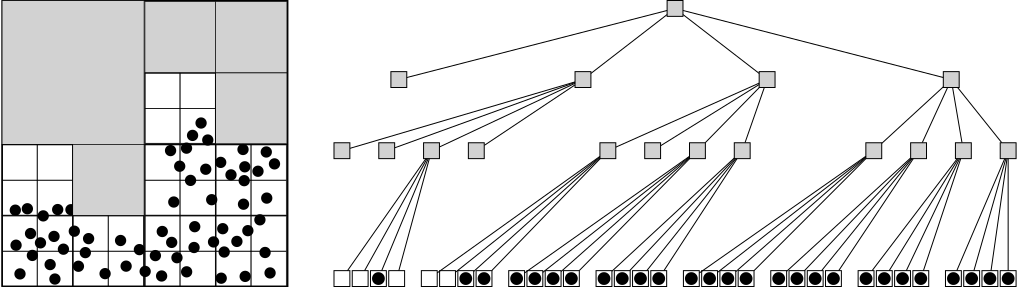
\includegraphics[width=\textwidth]{octree}
  \label{fig:octree}
  \caption[Quadtree-Veranschaulichung eines Octrees]{Quadtree (2d) zur Veranschaulichung der Funktionsweise eines Octrees (3d):\\
    Rekursive Unterteilung der interessanten Zellen bis zur gewünschten Auflösung, dann zellweises Binning
}
\end{figure}

Weitere Laufzeitoptimierungen ergeben sich bei Betrachtung der Addresszugriffe.
So wird bei der Ereignissuche wiederholt auf Zellen in direkter Nachbarschaft zugegriffen.
Durch Access Caching speichert man den letzten Zellzugriff und sucht bei weiteren Zugriffen auf dem Octree in der Nachbarschaft dieser Zelle, statt jede Zelladdressierung beim Root-Knoten zu beginnen.
Bei Aufruf einer leeren, nicht-allokierten Zelle speichert man stattdessen deren kleinste Superzelle, wodurch man automatisch die kleinste Superzelle der Nachbarschaft referenziert und folgende Suchoperationen signifikant verkürzt.
Addressierung der kleinsten gemeinsamen Superzelle geschieht durch Vergleich des höchsten unterschiedlichen Bits der Addresse, der auf einigen Prozessorarchitekturen fest im Chipsatz verankert ist und somit in konstanter Zeit läuft.

\todo[inline]{Wars das? Formeln?}

\subsection{k-d-Baum}

\begin{figure}[bthp]
  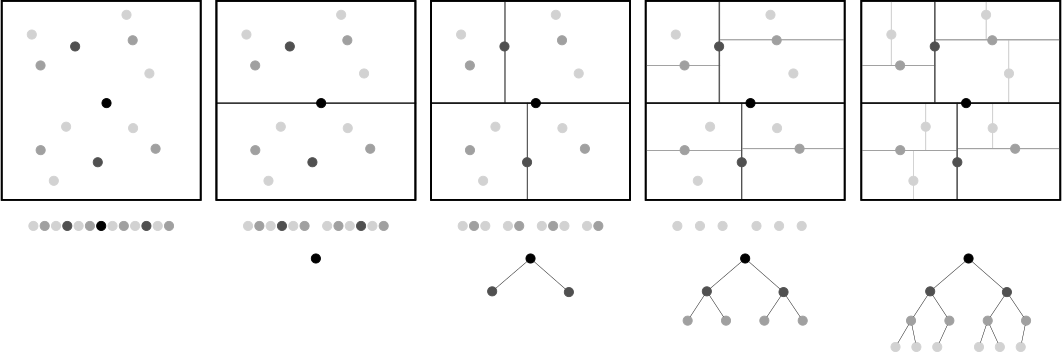
\includegraphics[width=\textwidth]{kdtree-tree}
  \caption[Konstruktion eines k-d-Baumes]{Konstruktion eines k-d-Baumes\todo[inline]{mehr Bildunterschrift}}
  \label{fig:kdtree}
\end{figure}

Sucht man nach optimalen Strukturen für Suchoperationen, stößt man schnell auf k-d-Bäume.
Diese unterteilen den gesamten Raum in Zellen, die jeweils genau ein Atom beinhalten.
Durch Algorithmus \ref{algo:kdtree-construction} zur Konstruktion eines k-d-Baumes ergibt sich ein balancierter Baum mit Atomen als Knoten, der als besondere Eigenschaft radiale Suchen nach beliebigen Punkten beschleunigt.
Ist ein Knoten weiter entfernt als eine vorherige Referenz, so sind dessen Kinder ebenfalls weiter entfernt.
Somit lässt sich per impliziter binärer Suche jedes nächste Atom in \BigO{\log{n}} finden.
In Verbindung mit einem Heap lässt sich auch eine feste Anzahl von Atomen in \BigO{\log{n}\log{N_r}}\todo{$N_r$?} suchen.

\begin{algorithm}
  \begin{algorithmic}
    \IF{N$\ge$1}
    \STATE Sortiere die Atome in Richtung der aktuellen Dimension (beginne mit x)
    \STATE Wähle Atom $\lfloor N/2 \rfloor$
    \STATE Teile Raum an $pos[d]_{\lfloor N/2 \rfloor}$ in zwei Zellen. Verteile die Atome auf beide Zellen.
    \STATE Wähle zyklisch die nächste Dimension
    \STATE Für beide Zellen: Gehe zu 1.
    \STATE kehre zurück
    \ENDIF
  \end{algorithmic}
  \caption[Konstruktion eines k-d-Baumes]{Konstruktion eines k-d-Baumes}
  \label{algo:kdtree-construction}
\end{algorithm}

Probleme von k-d-Bäumen zeigen sich bei der Suche nach einer Oberfläche einerseits und bei periodischen Räumen andererseits.

Die Oberfläche entlang einer Hauptachse lässt sich per Range Search mit anschließender Sortierung der Ergebnisse in \BigO{k\log{n^{1-\frac{1}{k}}}}\todo{REFERENZ!}{} ermitteln.
Möchte man jedoch das Auftreffen eines Precursors mit beliebiger Inklination ermitteln, kann man auf keine optimale Methode zurückgreifen.

Periodische Räume auf der anderen Seite brechen die Sucheigenschaften des k-d-Baumes, jedoch bloß am Rand der Struktur.
Nutzt man einen kleinen Suchbereich mit Radius $r$, der den Simulationsraum vollständig überlappt, so kann man die Periodizität vernachlässigen.
Andernfalls muss man entsprechend viele Suche in periodischen Bildern durchführen.
Die Modifikationsoperationen selbst bleiben unverändert.

Der größte Nachteil eines k-d-Baumes bleibt jedoch die Eigenschaft, beim Hinzufügen von Atomen beispielsweise entlang der z-Richtung stetig unbalancierter zu werden, wodurch Update-Operationen auf dem gesamten Baum notwendig wären.
Diese sind mit der geringen Konstruktionszeit zwar vertretbar, allerdings unnötig in Hinblick auf andere Methoden, wie Octrees und Delaunay-Triangulationen.

\subsection{Delaunay-Triangulation}

\CONTINUEHERE

\begin{figure}[bhpt]
  \centering
  \def\svgwidth{\textwidth}
  \input{img/delaunay.pdf_tex}
  \caption[Delaunay-Konstruktion]{Delaunay-Konstruktion}
  \label{fig:delaunay}
\end{figure}

Während bei den bisher vorgestellten Partitionsmethoden der Raum in k-dimensionale Quader geteilt wurde, basieren Triangulationen auf k-dimensionalen Simplexen, deren Eckpunkte die gespeicherte Punktmenge bilden.
Der Zentrale Vertreter ist die Delaunay-Triangulation, die für eine Menge von Punkten folgende Eigenschaften aufweist:

\begin{itemize}
\item Jeder Punkt ist ein Eckpunkt mindestens eines Simplexes
\item Simplexe überschneiden sich nicht
\item Innerhalb des Umkreises eines Simplexes befinden sich keine weiteren Punkte
\item Die Vereinigung aller Simplexe ergibt die konvexe Hülle
\item Ein Punkt teilt sich mit seinem nächsten Nachbarn mindestens einen Simplex \\
  $\Leftrightarrow$ Nächstnachbargraph $\subset$ Delaunay-Triangulation
  %% \item Die Delaunay-Triangulation und das Voronoi-Diagramm über die selben Punkte sind dual\\
  %% $\Rightarrow$ Allgemeine Nachbarschaftssuche ist \BigO{n\log n}
\end{itemize}

Eine Delaunay-Triangulation lässt sich aus einer Punktmenge in \BigO{n\log n}\todo{Referenz} ausführen, wofür eine Vielzahl an Algorithmen zur Verfügung stehen. \todo{Referenz}
Diesen liegt das Delaunay-Kriterium zu Grunde:
Der Umkreis eines Simplex' enthält nur seine eigenen Eckpunkte.
Ist dieses Kriterium bei zwei benachbarten Simplexen nicht gegeben, lässt sich per \textbf{Flip-Algorithmus} (Abbildung \ref{fig:delaunay-flip}) wieder eine Delaunay-Triangulation herstellen.
Dazu entfernt man die gemeinsame Kante bzw. Fläche der beiden betroffenen Simplexe und fügt zwischen den übrigen Punkten eine neue Grenze so ein, dass das Delaunay-Kriterium erfüllt ist.
Die dabei neu entstehenden Simplexe müssen nun mit ihren jeweiligen Nachbarn auf das Delaunay-Kriterium überprüft werden, wobei die neuen Simplexe als Bestandteil der Delaunay-Triangulation garantiert sind.\todo{Referenz}

\begin{figure}[bhpt]
  \captionsetup[subfigure]{singlelinecheck=false}{
    \def\subfigwidth{0.23\textwidth}
    \def\svgwidth{\textwidth}
    \begin{subfigure}[t]{\subfigwidth}
      \includegraphics[width=\textwidth]{delaunay-flip-a}
      \subcaption{Ausgangstriangulation}
      \label{fig:delaunay-flip-a}
    \end{subfigure}
    \hfill
    \begin{subfigure}[t]{\subfigwidth}
      \includegraphics[width=\textwidth]{delaunay-flip-b}
      \subcaption{Vereinigung invalider Simplexe}
      \label{fig:delaunay-flip-b}
    \end{subfigure}
    \hfill
    \begin{subfigure}[t]{\subfigwidth}
      \includegraphics[width=\textwidth]{delaunay-flip-c}
      \subcaption{Aufteilung in neue valide Simplexe}
      \label{fig:delaunay-flip-c}
    \end{subfigure}
    \hfill
    \begin{subfigure}[t]{\subfigwidth}
      \includegraphics[width=\textwidth]{delaunay-flip-d}
      \subcaption{Ergebnis}
      \label{fig:delaunay-flip-d}
    \end{subfigure}
  }
  \caption{Flip Algorithmus zur Aktualisierung einer Delaunay-Triangulation}
  \label{fig:delaunay-flip}
\end{figure}

\todo{Laufzeit Flipping?}

Für die Nachbarschaftssuche eines Referenzpunktes werden die raumfüllenden Eigenschaften der Triangulation relevant.
Der notwendigerweise konvexe, sonst aber beliebige Suchbereich um den Referenzpunkt wird von Simplexen überdeckt, die in direkter oder indirekter Nachbarschaft des Punktes liegen.
Somit teilen sich alle Punkte innerhalb des Suchbereiches eine Kante eines Simplexes mit einem anderen Punkt im Suchbereich.
Man muss nun einfach alle Kanten der Triangulation absuchen, bis man Punkte außerhalb des Suchbereiches findet.
Ein möglicher Algorithmus kann folgendermaßen aussehen:

\begin{algorithm}
  \centering
  \begin{algorithmic}
    \STATE Result = \{\}
    \STATE Queue = \{ P$_0$ : P$_0 \in$ Volume \}
    \WHILE{Queue $\neq \emptyset$}
    \STATE Sei P $\in$ Queue
    \STATE Queue = Queue $\setminus$ \{ P \}
    \IF{P $\in$ Volume}
    \STATE Result = Result $\cap$ \{ P \}
    \STATE Queue $\cap$ (Neighbors(P) $\setminus$ Result)
    \ENDIF
    \ENDWHILE
  \end{algorithmic}
  \caption[Nachbarschaftssuche auf einer Delaunay-Triangulation]{Nachbarschaftssuche auf einer Delaunay-Triangulation}
  \label{algo:delaunay-neighbors}
\end{algorithm}

\todo[inline]{continue here}

Dabei wird ausgenutzt, dass die Delaunay-Triangulation raumfüllend ist.
Somit werden nur Atome und Primitive untersucht, die Bestandteil des Suchraumes sind, weshalb diese Suche lokal und somit schnell bleibt.

Um die Position einzelner Punkte zu aktualisieren, arbeitet man üblicherweise mit Flip-Algorithmen, wie in Abbildung \ref{fig:delaunay-flip} dargestellt.

Hinsichtlich der Oberflächensuche wird allerdings eine andere Eigenschaft offensichtlich:
Die Alpha-Oberfläche ist ein Subgraph der Delaunay-Triangulation.
Vereinfacht ausgedrückt ist die Alpha-Form einer Punktmenge ihre ``ungefähre Form'', wie man sie wahrnehmen würde.
Oft zieht man auch Parallelen zum ``Einpacken in Plastikfolie mit Luftabpumpen''.
Die eigentliche Definition beinhaltet folgende Idee:

\begin{figure}[bhpt]
  \centering
  \captionsetup[subfigure]{singlelinecheck=false}{
    \def\subwidth{0.3\textwidth}
    \def\svgwidth{\textwidth}
    \begin{subfigure}[t]{\subwidth}
      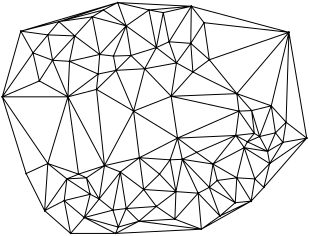
\includegraphics[width=\textwidth]{delaunay-alpha-a}
      \subcaption{Delaunay Triangulation}
      \label{fig:delaunay-alpha-a}
    \end{subfigure}
    \hfill
    \begin{subfigure}[t]{\subwidth}
      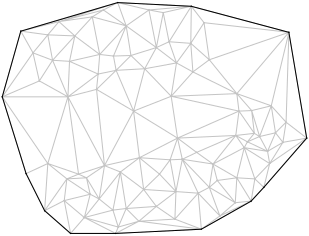
\includegraphics[width=\textwidth]{delaunay-alpha-b}
      \subcaption{Konvexe Hülle: Kanten mit nur einem Simplex}
      \label{fig:delaunay-alpha-b}
    \end{subfigure}
    \hfill
    \begin{subfigure}[t]{\subwidth}
      \includegraphics[width=\textwidth]{delaunay-alpha-c}
      \subcaption{Alpha-Form: Hülle nach Entfernung von Simplexen mit $\text{Umkreis} > \alpha$}
      \label{fig:delaunay-alpha-c}
    \end{subfigure}
  }
  \caption{Konstruktion einer Alpha-Form}
  \label{fig:delaunay-alpha}
\end{figure}

Entfernt man alle Delaunay-Primitive, deren Umkreisradius oberhalb eines Grenzwertes $\alpha$ liegt, und bildet dann die Vereinigung aller verbleibenden Primitive sowie etwaiger frei gewordener Punkte, so erhält man die Alphaform.
Für $\alpha = \infty$ erhält man somit die konvexe Hülle.
Für endliche Werte von $\alpha$ hingegen werden auch konkave Bereiche in der Oberfläche betrachtet.
Wählt man $\alpha$ jedoch unterhalb des kleinsten Abstandes der Atome, so erfasst man zwangsläufig auch Atome im Inneren der Struktur, wodurch die Idee der allgemeinen Oberfläche wieder verloren geht.

Verwaltet man nun parallel zur Delaunay-Triangulation eine Liste der theoretisch durch den $alpha$-Algorithmus entfernten Primitive, so hat man die Oberfläche der gesamten Struktur charakterisiert, ohne nennenswerten Mehraufwand treiben zu müssen.
Durch Kenntnis dieser Oberfläche ließen sich nun CVD-Prozesse auch an spitzen Strukturen betrachten, ohne dem Wachstum die Charakteristika der räumlichen Darstellung aufzuzwingen.

Bisher ist es jedoch bei theoretischen Betrachtungen dieser Delaunay-basierten Methoden geblieben.
Hinsichtlich allgemeiner Oberflächensimulationen ließe sich diese Methode der Delaunay-Triangulationen perspektivisch in Parsivald einpflegen.
